
	\documentclass{article}
	\usepackage{amsmath,amssymb}
	\usepackage[inline]{enumitem}
	\usepackage{blindtext}
	\usepackage{booktabs}
	\usepackage{graphicx}
	\usepackage{xcolor}
	\usepackage[vmargin = 1.5in, top = 1in, bottom = 1.2in, letterpaper]{geometry}
	\usepackage{listings}
	\usepackage{courier}
	\usepackage{multicol}
	\usepackage{multirow}
	\usepackage{bm}
	\usepackage{subcaption}
	\usepackage{tabularx}
	\lstset{
	basicstyle = \small\tt,
	keywordstyle = \tt\color{blue},
	commentstyle = \it\color[cmyk]{1,0,1,0},
	stringstyle = \tt\color[RGB]{128,0,0},
	%frame = single,
	backgroundcolor = \color[RGB]{245,245,244},
	breaklines,
	extendedchars = false,
	xleftmargin = 2em,
	xrightmargin = 2em,
	aboveskip = 1em,
	tabsize = 4,
	showspaces = false
	}
	\begin{document}
	
	% \newfontfamily\courier{Courier New}

	
	\title{STAT 557 Homework 3}
	\author{Yifan Zhu}
	\maketitle
	
	\begin{enumerate}[leftmargin = 0 em, label = \arabic*., font = \bfseries]
	\item 
	\begin{enumerate}
		\item 
		Under the alternative hypothesis, $\hat{m}_{A, ij} = Y_{ij}$. 

		Under the null hypothesis, 
		\begin{align*}
		\hat{m}_{0,i1} = \frac{9}{16}n_i\\
		\hat{m}_{0,i2} = \frac{3}{16}n_i\\
		\hat{m}_{0,i3} = \frac{3}{16}n_i\\
		\hat{m}_{0,i4} = \frac{1}{16}n_i\\
		\end{align*}
		where $n_i = \sum_{j=1}^4 Y_{ij}$. 

		Thus we have 
		\[G^2 = 2\sum_{i=1}^3 \sum_{j=1}^4 Y_{ij} \log (\hat{m}_{A,ij}/\hat{m}_{0,ij}) = 3.143858\]

		The degrees of freedom is \textbf{9} and p-value is \textbf{0.9583171}. With large p-value we conclude that the model fits the data well.
		

		\item
		Let the parameters for multinomial distribution be region $i$ be $p_{ai}p_{bi}, (1 - p_{ai})p_{bi}, p_{ai}(1-p_{bi}), (1 - p_{ai})(1 - p_{bi})$. Then 
		\begin{align*}
		 \ell &= \sum_{i=1}^3 \log n_i! \\
		 & + \sum_{i=1}^3 \left[Y_{i1} \log (p_{ai}p_{bi}) + Y_{i2}\log((1 - p_{ai})p_{bi}) + Y_{i3}\log(p_{ai}(1 - p_{bi})) + Y_{i4}\log( (1 - p_{ai})(1 - p_{bi}))\right]\\
		 & - \sum_{i=1}^3 \sum_{j=1}^4 \log Y_{ij}!
		 \end{align*} 

		 Let $\frac{\partial \ell}{\partial p_{ai}} =  \frac{\partial \ell}{\partial p_{bi}} = 0$, we have
		 \[\hat{p}_{ai} = \frac{Y_{i1} + Y_{i3}}{n_i}, \hat{p}_{bi} = \frac{Y_{i1} + Y_{i2}}{n_i} \]

		 And 
		 \begin{align*}
		 &\hat{m}_{0, i1} = \hat{p}_{ai} \hat{p}_{bi} n_i\\
		 &\hat{m}_{0, i2} = (1 - \hat{p}_{ai})\hat{p}_{bi} n_i \\
		 &\hat{m}_{0, i3} = \hat{p}_{ai}(1 - \hat{p}_{bi}) n_i\\
		 &\hat{m}_{0, i4} = (1 - \hat{p}_{ai})(1 - \hat{p}_{bi}) n_i
		 \end{align*}

		 Then 
		 \[G^2 = 1.133048\]
		 The degrees of freedom is \textbf{3} and the p-value is \textbf{0.7691027}. With large p-value we conclude that the model fits the data well.
		 
		\item 
		Set $p_{ai} = p_{a}$ for $i = 1,2,3$, then we have
		\begin{align*}
		 \ell &= \sum_{i=1}^3 \log n_i! \\
		 & + \sum_{i=1}^3 \left[Y_{i1} \log (p_{a}p_{b}) + Y_{i2}\log((1 - p_{a})p_{b}) + Y_{i3}\log(p_{a}(1 - p_{b})) + Y_{i4}\log( (1 - p_{a})(1 - p_{b}))\right]\\
		 & - \sum_{i=1}^3 \sum_{j=1}^4 \log Y_{ij}!
		 \end{align*} 
		 Let $\frac{\partial \ell}{\partial p_{a}} =  \frac{\partial \ell}{\partial p_{b}} = 0$, we have
		 \[\hat{p}_{a} = \frac{\sum_{i=1}^3 (Y_{i1} + Y_{i3})}{n}, \hat{p}_{b} = \frac{\sum_{i=1}^3 (Y_{i1} + Y_{i2})}{n} \]
		 where $n = \sum_{i=1}^3 n_i = \sum_{i=1}^3 \sum_{j=1}^4 Y_{ij}$.
		 Then 
		 \[G^2 = 1.628537\]
		 The degrees of freedom is \textbf{7} and the p-value is \textbf{0.9775233}. With large p-value we conclude that the model fits the data well.
		\item  Let the model for (a), (b), (c) be Model A, Model B and Model C. And the model for alternative hypothesis be the saturated model Model S, then parameter space of Model A is in Model C in Model B in Model S. The deviance table is shown below

		\begin{center}
		\begin{tabular}{llll}
				\textbf{Comparison} & \textbf{d.f.} &\textbf{deviance value} & \textbf{p-value}\\
				\midrule
				Model A vs Model C & 2  & 1.515321 & 0.4687618\\
				Model C vs Model B & 4 &  0.4954887 & 0.9739387\\
				Model B vs Model S & 3 &  1.133048 & 0.7691027\\
				\midrule
				Model A vs Model S & 9 & 3.143858 & 0.9583171		
		\end{tabular}
		\end{center}
		 From the table we see Model A already fit the data pretty well, and finer models do not fit significantly better. Thus we can use Model A.
		 \item 
		 Model A, B and C all provide an adequate description of the data. The simplest one is Model A. Large p-value shows a good fit of data and finer models do not fit significantly better because of the large p-value.
	\end{enumerate}

	\item 
	\[f(y_i| \mu) = \frac{\mu^{y_i}}{y_i !} \mathrm{e}^{-\mu}\]
	then
	\[\ell = \log \prod_{i=1}^n f(y_i | \mu) = \log \mu \sum_{i=1}^n y_i - n \mu - \sum_{i=1}^n \log y_i! = n \bar{y} \log \mu - n \mu - \sum_{i=1}^n \log y_i!\]
	where $\bar{y} = \frac{1}{n} \sum_{i=1}^n y_i$. Then
	\begin{align*}
	& \frac{\partial \ell}{\partial \mu} = \frac{n \bar{y}}{\mu} - n = Q\\
	& \frac{\partial^2 \ell}{\partial \mu^2} = - \frac{n \bar{y}}{\mu^2} = - H
	\end{align*}
	Hence
	\[I = E[H] = E\left[-\frac{\partial^2 \ell}{\partial \mu^2}\right] = \frac{n Ey_i}{\mu^2} = \frac{n}{\mu}\]

	Using Fisher scoring algorithm, 
	\[\hat{\mu}^{(1)} = \hat{\mu}^{(0)} +[ \hat{I}^{(0)}]^{-1} \hat{Q}^{(0)} = \hat{\mu}^{(0)} + \frac{\hat{\mu}^{(0)}}{n} \left(\frac{n \bar{y}}{\hat{\mu}^{(0)}} - n\right) = \bar{y}\]
	Now 
	\[\hat{Q}^{(1)} = \frac{n \bar{y}}{\hat{\mu}^{(1)}} - n = 0\]
	thus it converges after one step.

	Using Newton-Raphson, we have
	\[\hat{\mu}^{(s+1)} = \hat{\mu}^{(s)} + [\hat{H}^{(s)}]^{-1} \hat{Q}^{(s)} = \hat{\mu}^{(s)} + \frac{{(\hat{\mu}^{(s)}})^2}{n \bar{y}}\left(\frac{n \bar{y}}{\hat{\mu}^{(s)}} - n\right) = 2 \hat{\mu}^{(s)} - \frac{(\hat{\mu}^{(s)})^2}{\bar{y}}\]
	Then
	\[\hat{\mu}^{(s+1)} - \hat{\mu}^{(s)} = \left[ 2 - \frac{\hat{\mu}^{(s+1)}+\hat{\mu}^{(s)}}{\bar{y}}\right](\hat{\mu}^{(s)} - \hat{\mu}^{(s-1)})\]
	Because 
	\[\hat{\mu}^{(s+1)} = 2 \hat{\mu}^{(s)} - \frac{(\hat{\mu}^{(s)})^2}{\bar{y}} = -\frac{1}{\bar{y}}(\hat{\mu}^{(s)} - \bar{y})^2 + \bar{y}\]
	when 0 < $\hat{\mu}^{(0)} < 2 \bar{y}$, we have $0 < \hat{\mu}^{(s)} \leq \bar{y}$. Then 
	\[\left|2 - \frac{\hat{\mu}^{(s+1)}+\hat{\mu}^{(s)}}{\bar{y}}\right| \leq 1, \forall s \geq 1\]
	Hence with initial value $\hat{\mu}^{(0)} \in (0, 2 \bar{y})$, Newton-Raphson converges. When $\hat{\mu}^{(0)} > 2 \bar{y}$, we have $\hat{\mu}^{(1)} < 0$. Then it does not converge. 

	\item 
	\begin{enumerate}
		\item 
		\[f(y|k, \mu) = \exp(\log f(y| k, \mu))\]
		and
		\begin{align*}
		\log f(y| k, \mu) &= \log \Gamma(y + k) - \log \Gamma(k) - \log G(y+1) + k \log k - k \log(\mu + k) + y\left(\log (1 - \frac{k}{\mu + k})\right)\\
		& = y \log \left( 1 - \frac{k}{\mu + k}\right)  - \log ( \mu + k) + [k \log k + \log \Gamma (y + k) - \log \Gamma(k) - \log \Gamma(y + 1)]
		\end{align*}

		Here $T(\mu) = \log \left( 1 - \frac{k}{\mu + k}\right),\, A(\mu) = \log ( \mu + k),\, h(y) = k \log k + \log \Gamma (y + k) - \log \Gamma(k) - \log \Gamma(y + 1)$. $f(t|k, \mu) = \exp(y T(\mu) - A(\mu) + h(y))$.It is a member of the exponential family.
		
		\item It is not a member of exponential family. Because in this case $log \Gamma (y + k)$ cannot be expressed as $y g(\mu, k)$ for some function $g$. Hence it is not a member of exponential family.
	\end{enumerate}

	\item 
	\begin{enumerate}
		\item 
	Estimates and standard errors of $\beta_0$ and $\beta_1$ is shown below.
	\begin{center}
	\begin{tabular}{lll}
	\toprule
	 \textbf{Parameter} &\textbf{Estimate} &\textbf{Standard Error}\\ 
     \midrule
     $\beta_0$ &-61.3183 &12.0224 \\
     $\beta_1$ &2.2110   &0.4309\\ 
 	\bottomrule
	\end{tabular}
	\end{center}
	\item 
	The Wald Chi-squared statistic is given by 
	\[\frac{(\hat{\beta}_1^2)}{\widehat{Var}(\hat{\beta}_1)} = 26.3345\]
	The degrees of freedom is 1 and p-value is $< 0.0001$. With small p-value we reject the null hypothesis and conclude that there is significant evidence that $\beta_1 \neq 0$ and the expected proportion of female born is non-constant with respect to the incubation temperature.
	
	\item 
	The odds ratio is estimated by
	\[\mathrm{e}^{\hat{\beta}_1} = 9.125\]
	And the confidence interval is to plug in confidence interval of $\hat{\beta}_1$ to $\exp(\cdot)$. The 95\% confidence interval is 
	\[(3.922, 21.232)\]


	\item 
	Let 
	\[\eta = \beta_0 + 28 \beta_1\]
	And we have
	\[\log\left(\frac{\pi}{1 - \pi}\right) = \eta \Rightarrow \pi = \frac{\mathrm{e}^{\eta}}{1 + \mathrm{e}^{\eta}}\]
	Then the estimate would be 
	\begin{align*}
	& \hat{\eta} = \hat{\beta}_0 + 28 \hat{\beta}_1 = 0.5897\\
	& \hat{\pi} = \frac{\mathrm{e}^{\hat{\eta}}}{1 + \mathrm{e}^{\hat{\eta}}} = 0.6433
	\end{align*}

	Using Delta Method to obtain the standard error of $\hat{\pi}$.
	\begin{align*}
	 & \frac{\partial \pi}{\partial \beta_0} = \frac{\partial \pi}{\partial \eta}\frac{\partial \eta}{\partial \beta_0} = \frac{\mathrm{e}^\eta}{(1 + \mathrm{e}^\eta)^2}\\
	 & \frac{\partial \pi}{\partial \beta_1} = \frac{\partial \pi}{\partial \eta}\frac{\partial \eta}{\partial \beta_1} = \frac{28\mathrm{e}^\eta}{(1 + \mathrm{e}^\eta)^2}\\
	 \end{align*}
	 Let
	 \[D = \begin{bmatrix}
	 	\frac{\partial \pi}{\partial \beta_0} & \frac{\partial \pi}{\partial \beta_1}
	 \end{bmatrix}\]
	 then $\hat{D} = D|_{\eta = \hat{\eta}}$ and
	 \[\widehat{Var}(\pi) = \hat{D}\widehat{Var}([\hat{\beta}_0\, \hat{\beta}_1])\hat{D}^T = 0.0027\]
	 and
	 \[s.e.(\hat{\pi}) = \sqrt{\widehat{Var}(\hat{\pi)}} = 0.052\]

	 \item 
	When $\pi = 0.5$, we have
	\[0 = \beta_0 + t \beta_1 \Rightarrow t = -\frac{\beta_0}{\beta_1}\]
	Then the estimate
	\[\hat{t} = -\frac{\hat{\beta}_0}{\hat{\beta}_1} = 27.7333\]
	Using Delta Method to obtain the standard error of $\hat{t}$.
	\begin{align*}
	 & \frac{\partial t}{\partial \beta_0} = -\frac{1}{\beta}_1\\
	 & \frac{\partial t}{\partial \beta_1} = \frac{\beta_0}{\beta_1^2}\\
	 \end{align*}
	 Let
	 \[D = \begin{bmatrix}
	 	\frac{\partial t}{\partial \beta_0} & \frac{\partial t}{\partial \beta_1}
	 \end{bmatrix}\]
	 then $\hat{D} = D|_{\beta_0= \hat{\beta}_0, \beta_1 = \hat{\beta}_1}$ and
	 \[\widehat{Var}(\hat{t}) = \hat{D}\widehat{Var}([\hat{\beta}_0\, \hat{\beta}_1])\hat{D}^T = 0.0111582\]
	 and
	 \[s.e.(\hat{t}) = \sqrt{\widehat{Var}(\hat{t})} = 0.1056324\]
	 Hence the 95\% confidence interval is
	 \[(\hat{t} - 1.96 s.e.(\hat{t}), \hat{t} + 1.96 s.e.(\hat{t})) = (27.52625, 27.94033)\]

	 \item 
	 The plot is shown below
	 \begin{center}
	 	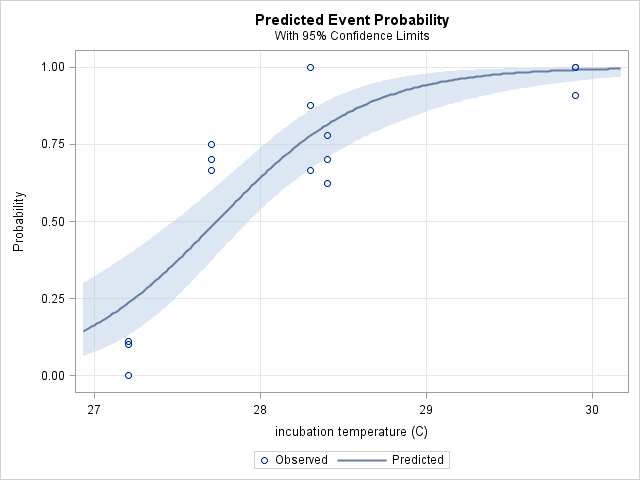
\includegraphics[width = 0.6\textwidth]{EffectPlot.png}
	 \end{center}

	 And the Hosmer-Lemeshow test chi-squared statistic is \textbf{14.9522}. The degrees of freedom is 3 and the p-value is \textbf{0.0019}. The p-value is small and we tend to say the fit is not good. From the plot we can also know the fit is not quite good.

	 	  \item 
	 	  For \verb|teggnm.txt|, estimates and standard errors of $\beta_0$ and $\beta_1$ is shown below.
	\begin{center}
	\begin{tabular}{lll}
	\toprule
	 \textbf{Parameter} &\textbf{Estimate} &\textbf{Standard Error}\\ 
     \midrule
     $\beta_0$ &-41.7419 & 14.5197\\
     $\beta_1$ &1.4696   &0.5126\\ 
 	\bottomrule
	\end{tabular}
	\end{center}

	\item 
	Repeat what we did in (e). When $\pi = 0.5$, we have
	\[0 = \beta_0 + t \beta_1 \Rightarrow t = -\frac{\beta_0}{\beta_1}\]
	Then the estimate
	\[\hat{t} = -\frac{\hat{\beta}_0}{\hat{\beta}_1} = 28.40358\]
	Using Delta Method to obtain the standard error of $\hat{t}$.
	\begin{align*}
	 & \frac{\partial t}{\partial \beta_0} = -\frac{1}{\beta}_1\\
	 & \frac{\partial t}{\partial \beta_1} = \frac{\beta_0}{\beta_1^2}\\
	 \end{align*}
	 Let
	 \[D = \begin{bmatrix}
	 	\frac{\partial t}{\partial \beta_0} & \frac{\partial t}{\partial \beta_1}
	 \end{bmatrix}\]
	 then $\hat{D} = D|_{\beta_0= \hat{\beta}_0, \beta_1 = \hat{\beta}_1}$ and
	 \[\widehat{Var}(\hat{t}) = \hat{D}\widehat{Var}([\hat{\beta}_0\, \hat{\beta}_1])\hat{D}^T = 0.09115882\]
	 and
	 \[s.e.(\hat{t}) = \sqrt{\widehat{Var}(\hat{t})} = 0.3019252\]
	 Hence the 95\% confidence interval is
	 \[(\hat{t} - 1.96 s.e.(\hat{t}), \hat{t} + 1.96 s.e.(\hat{t})) = (27.81181, 28.99535)\]


	 \item 
	 From the results above we have
	 \[\hat{t}_{il} - \hat{t}_{nm} = -0.6702911\]
	 and
	 \[\widehat{Var}(\hat{t}_{il} - \hat{t}_{nm}) = \widehat{Var}({\hat{t}_{il}}) + \widehat{Var}(\hat{t}_{nm}) = 0.102317\]
	 So the asymptotic normal test statistic is
	 \[z = \frac{\hat{t}_{il} - \hat{t}_{nm}}{\sqrt{\widehat{Var}({\hat{t}_{il}}) + \widehat{Var}(\hat{t}_{nm})}} = -2.095509\] 
	 and the absolute value $|z|$ is greater than 1.96. Hence we fail to reject the null hypothesis and conclude that there is no significant difference between the incubation temperature at with 50\% of the eggs produce females for Illinois and New Mexico.

	 \item 
	 Using the logit and complimentary log-log link, we get the AIC and BIC for Illinois and New Mexico. The results are shown below.

	 Illinois:

	 \begin{center}
	   	\begin{tabular}{lll}
	   	\toprule
	   	 & AIC & BIC\\
	   	 \midrule
   logit & 53.836 & 59.662\\
   cloglog &  61.8852 & 63.3013\\
   \bottomrule
	   	\end{tabular}
	   \end{center}  

	 New Mexico:
	 \begin{center}
	   	\begin{tabular}{lll}
	   	\toprule
	   	 & AIC & BIC\\
	   	 \midrule
   logit & 26.866 & 29.798\\
   cloglog &  28.5217 & 28.9161\\
   \bottomrule
	   	\end{tabular}
	   \end{center}  
	
	For Illinois, the AIC and BIC are both higher when using complementary log-log link, thus it is not a better model than logistic regression. For New Mexico, the AIC is a bit higher and BIC is a bit lower when using complementary log-log. So it is not a better model than logistic regression for New Mexico either.


	\item 
    We use a link function like
    \[\log\left(\frac{(1 - \pi)^{- \alpha}-1}{\alpha}\right)\]
    and set $\alpha = 10$. 
	The AIC and BIC for Illinois and New Mexico using this model is 
	\begin{center}
		\begin{tabular}{lll}
		 \toprule
		 & AIC & BIC\\
		 \midrule
		 Illinois & 45.7833 & 47.1994\\
		 New Mexico & 22.4850 & 22.8794\\
		 \bottomrule
		\end{tabular}
	\end{center}
	We can see AIC and BIC are both smaller using this model, so it should be better in describing the data. 

	Furthermore, the fitted curve seems to fit the data better with this model compared to the logistic regression.

	Illinois:
	\begin{center}
		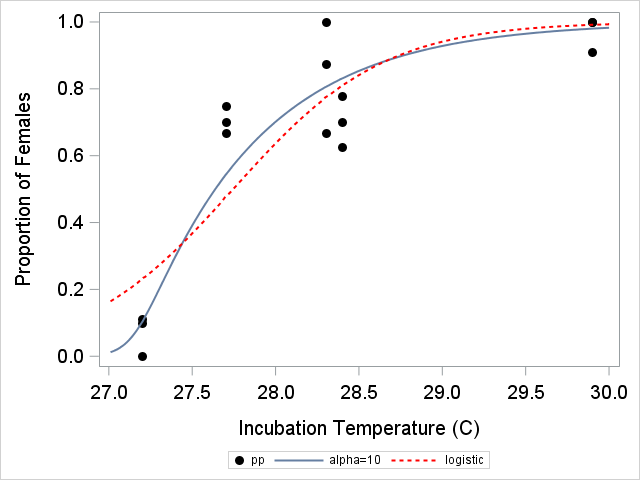
\includegraphics[width = 0.6\textwidth]{SGPlot4il.png}
	\end{center}

	New Mexico:
	\begin{center}
		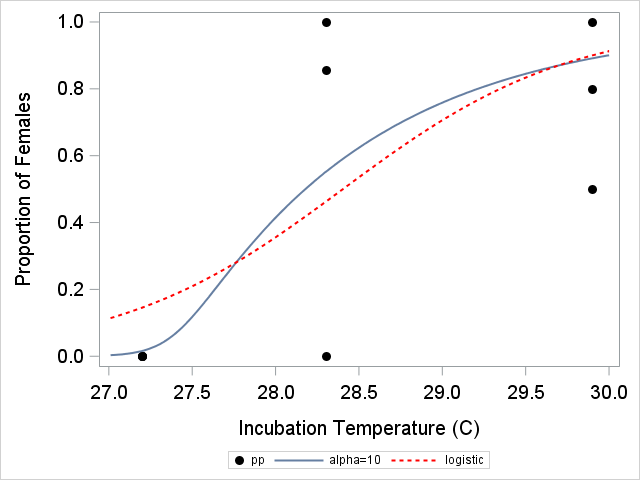
\includegraphics[width = 0.6\textwidth]{SGPlot3nm.png}
	\end{center}

	Similar to what we did in (e),
	When $\pi = 0.5$, we have
	\[\eta_0 = \beta_0 + t \beta_1 \Rightarrow t = \frac{\eta_0 - \beta_0}{\beta_1}\]
	where 
	\[\eta_0 = \log\left(\frac{2^{10}  -1}{10}\right)\]
	Then the estimate
	\[\hat{t} = -\frac{\hat{\beta}_0}{\hat{\beta}_1}\]
	Using Delta Method to obtain the standard error of $\hat{t}$.
	\begin{align*}
	 & \frac{\partial t}{\partial \beta_0} = -\frac{1}{\beta}_1\\
	 & \frac{\partial t}{\partial \beta_1} = \frac{\beta_0 - \eta_0}{\beta_1^2}\\
	 \end{align*}
	 Let
	 \[D = \begin{bmatrix}
	 	\frac{\partial t}{\partial \beta_0} & \frac{\partial t}{\partial \beta_1}
	 \end{bmatrix}\]
	 then $\hat{D} = D|_{\beta_0= \hat{\beta}_0, \beta_1 = \hat{\beta}_1}$ and
	 \[\widehat{Var}(\hat{t}) = \hat{D}\widehat{Var}([\hat{\beta}_0\, \hat{\beta}_1])\hat{D}^T \]
	 and
	 \[s.e.(\hat{t}) = \sqrt{\widehat{Var}(\hat{t})}\]
	 Hence the 95\% confidence interval is
	 \[(\hat{t} - 1.96 s.e.(\hat{t}), \hat{t} + 1.96 s.e.(\hat{t}))\]

	 The estimates and confidence interval for Illinois and New Mexico is shown in the table below.
	 \begin{center}
	 	\begin{tabular}{lll}
	 	\toprule
	 	 & Estimate & 95\% CI\\
	 	 \midrule
	 	 Illinois & 27.63837 & (27.50222, 27.77453)\\
	 	 New Mexico & 28.17839 & (27.67799, 28.67880) \\
	 	 \bottomrule
	 	\end{tabular}
	 \end{center}
	\end{enumerate}

	\item 
	\begin{enumerate}
		\item 
		$\omega$ is the proportion of people that never drink water in population. $\mu$ is the mean milk consumption in people that drink milk in population.

		 \item 
		 \begin{align*}
		  E(X) &= \sum_{x = 0}^\infty x P(X = x) = 0 \cdot  \omega + (1 - \omega) \sum_{x = 0}^\infty x \frac{\mathrm{e}^{-\mu} \mu^{x}}{x!} = (1 - \omega)\mu\\
		  E(X^2) & = \sum_{x = 0}^\infty x^2 P(X = x) = 0^2 \cdot \omega + (1 - \omega) \sum_{x = 0}^\infty x^2 \frac{\mathrm{e}^{-\mu} \mu^{x}}{x!} = (1 - \omega)(\mu^2 + \mu)\\
		  Var(X) &= E(X^2) - (E(X))^2 = (1 - \omega)(\omega \mu^2 + \mu)
		  \end{align*}

		  \item 
		  $\log \mu = \eta_1,\, \log(\omega) = \eta_2$. Thus $\mu = \exp(\eta_1), \omega = \exp(\eta_2)$. And we have
		  \begin{align*}
		   &\hat{\eta}_1 = 0.3388\\
		   & \hat{\eta}_2 = -1.5638\\
		   &s.e.(\hat{\eta}_1) = 0.0296\\
		   & s.e.(\hat{\eta}_2) = 0.0877
		   \end{align*}
		   Hence 
		   \begin{align*}
		   &\hat{\mu} = \exp(\hat{\eta_1}) = 1.403263\\
		   &s.e.(\hat{\mu}) = \left|\frac{\partial \mu}{\partial \eta_1}\right|_{\eta_1 = \hat{\eta_1}} s.e.(\hat{\eta}_1) = 0.04148793\\
		   &\hat{\omega} = \exp(\eta_2) = 0.2093341 \\
		   &s.e.(\hat{\omega}) = \left|\frac{\partial \omega}{\partial \eta_2}\right|_{\eta_2 = \hat{\eta_2}} s.e.(\hat{\eta}_2) = 0.01835863 
		   \end{align*}


		   \item 
		   The mean consumption is
		   \[m = (1 - \omega) \mu\]
		   Then we have
		   \[\hat{m} = (1 - \hat{\omega}) \hat{\mu} = 1.109474 \]
		   And
		   \begin{align*}
		    &\frac{\partial m}{\partial \eta_1} = \frac{\partial m}{\partial \mu} \frac{\partial \mu}{\partial \eta_1} = (1 - \omega) \exp(\eta_1) = (1 - \omega) \mu\\
		    & \frac{\partial m}{\partial \eta_2} = \frac{\partial m}{\partial \omega} \frac{\partial \omega}{\partial \eta_2} = -\mu \exp(\eta_2) = -\mu \omega
		    \end{align*}
		    Let $D = \begin{bmatrix}
		    	\frac{\partial m}{\partial \eta_1}&\frac{\partial m}{\partial \eta_2}
		    \end{bmatrix}$, then by Delta Method
		    \[s.e.(\hat{m}) = \sqrt{D\widehat{Var}([\hat{\eta}_1\, \hat{\eta_2}])D^T} = 0.0274856\]
		    Hence 95\% confidence interval is
		    \[(\hat{m} - 1.96 s.e.(\hat{m}), \hat{m} + 1.96 s.e. (\hat{m})) = (1.055602, 1.163345)\]

		    \item 
            The probability is
		   \[p = P(X = 0) = \omega + (1 - \omega)\mathrm{e}^{-\mu}\]
		   Then we have
		   \[\hat{p} = \hat{\omega} + (1 -\hat{\omega}) \mathrm{e}^{-\hat{\mu}} = 0.4036842  \]
		   And
		   \begin{align*}
		    &\frac{\partial p}{\partial \eta_1} = \frac{\partial p}{\partial \mu} \frac{\partial \mu}{\partial \eta_1} = -(1 - \omega)\mathrm{e}^{-\mu} \exp(\eta_1) = -(1 - \omega)\mathrm{e}^{-\mu}\mu\\
		    & \frac{\partial p}{\partial \eta_2} = \frac{\partial p}{\partial \omega} \frac{\partial \omega}{\partial \eta_2} = -(1 - \exp(-\mu)) \exp(\eta_2) = (1 - \exp(-\mu)) \omega
		    \end{align*}
		    Let $D = \begin{bmatrix}
		    	\frac{\partial m}{\partial \eta_1}&\frac{\partial m}{\partial \eta_2}
		    \end{bmatrix}$, then by Delta Method
		    \[s.e.(\hat{p}) = \sqrt{D\widehat{Var}([\hat{\eta}_1\, \hat{\eta_2}])D^T} = 0.01125595\]
		    Hence 95\% confidence interval is
		    \[(\hat{p} - 1.96 s.e.(\hat{p}), \hat{p} + 1.96 s.e. (\hat{p})) = (0.3816226, 0.4257459)\]

		    \item 
		    The proportion of population that never drinks milk is $\omega$, thus the 95\% confidence interval is
		    \[(\hat{\omega} - 1.96 s.e.(\hat{\omega}) , \hat{\omega} + 1.96 s.e.(\hat{\omega}) ) = (0.1733512, 0.2453170 )\]

		    \item 
		    When fitting the Poisson model, the last category has a expected value less than 2, thus we need to combine it with category corresponding to number of glasses being 5 and then compute the Pearson statistic. The chi-squared statistic is then \textbf{153.7398}, degrees of freedom is \textbf{4} and p-value is $< \textbf{0.0001}$. 

		    Fitting the ZIP model, the last category then has a expected value of 4.8, which is close to 5. So we did not combine categories in this case. The chi-squared statistic is \textbf{38.04},  degrees of freedom is \textbf{4} and p-value is $< \textbf{0.0001}$. 


		     
		   
		    

		   
	\end{enumerate}

	\item 
	\begin{enumerate}
		\item 
		$\pi$ is the probability that a person randomly selected from the mixture of populations gives a zero response. $\mu$ does not have a clear meaning in the context.
		\item 
		\begin{align*}
		& E(X) = \frac{1 - \pi}{1 - \mathrm{e}^{-\mu}} \sum_{x = 1}^\infty x\frac{\mathrm{e}^{-\mu} \mu^x}{\Gamma(x+1)} = \frac{(1 - \pi)\mu}{1 - \mathrm{e}^{- \mu}}\\
		& E(X^2) = \frac{1 - \pi}{1 - \mathrm{e}^{-\mu}} \sum_{x = 1}^\infty x^2\frac{\mathrm{e}^{-\mu} \mu^x}{\Gamma(x+1)} = \frac{(1 - \pi)(\mu + \mu^2)}{1 - \mathrm{e}^{- \mu}}\\
		& Var(X) = E(X^2) - (E(X))^2 = \left(\frac{1 - \pi}{1 - \mathrm{e}^{-\mu}}\right)\left(\mu + \left(\frac{\pi - \mathrm{e}^{-\mu}}{1 - \mathrm{e}^{-\mu}}\right)\mu^2\right)
		\end{align*}

		\item 
		$\log \mu = \eta_1,\, \log(\pi /(1 - \pi)) = \eta_2$. Thus $\mu = \exp(\eta_1), \pi = 1/(1 +\exp(-\eta_2))$.  And we have
		  \begin{align*}
		   &\hat{\eta}_1 = 0.3388\\
		   & \hat{\eta}_2 = -0.3901\\
		   &s.e.(\hat{\eta}_1) = 0.02957\\
		   & s.e.(\hat{\eta}_2) = 0.04676
		   \end{align*}
		   Hence 
		   \begin{align*}
		   &\hat{\mu} = \exp(\hat{\eta_1}) = 1.4032\\
		   &s.e.(\hat{\mu}) = \left|\frac{\partial \mu}{\partial \eta_1}\right|_{\eta_1 = \hat{\eta_1}} s.e.(\hat{\eta}_1) = 0.04149\\
		   &\hat{\pi} = 1/(1+\exp(-\eta_2)) = 0.4037 \\
		   &s.e.(\hat{\pi}) = \left|\frac{\partial \pi}{\partial \eta_2}\right|_{\eta_2 = \hat{\eta_2}} s.e.(\hat{\eta}_2) = 0.01126 
		   \end{align*}

		   \item 
		   The 95\% confidence interval for $\hat{\pi}$ is
		   \[(0.3771, 0.4303)\]

		   \item 
		   This is not a estimable quantity.

		   \item 
		   Fitting the Poisson Hurdle model, the last category then has a expected value of 4.8, which is close to 5. So we did not combine categories in this case. The chi-squared statistic is \textbf{38.04},  degrees of freedom is \textbf{4} and p-value is $< \textbf{0.0001}$. 

		
	\end{enumerate}
	

	\item 
	\begin{enumerate}
		\item 
		$\omega$ is the proportion of people that never drink water in population. $\mu$ is the mean milk consumption in people that drink milk in population.

		 \item 
		 \begin{align*}
		  E(X) &= (1 - \omega) \mu\\
		  Var(X) &= (1 - \omega)[\mu(1 + \mu \kappa)+ \omega \mu^2]
		  \end{align*}

		  \item 
		  $\log \mu = \eta_1,\, \log(\omega /(1 - \omega)) = \eta_2$. Thus $\mu = \exp(\eta_1), \omega = 1/(1 +\exp(-\eta_2))$. $\kappa$ is still $\kappa$. And we have
		  \begin{align*}
		   &\hat{\eta}_1 = 0.1962\\
		   & \hat{\eta}_2 = -2.3358\\
		   &s.e.(\hat{\eta}_1) = 0.0561\\
		   & s.e.(\hat{\eta}_2) = 0.5752
		   \end{align*}
		   Hence 
		   \begin{align*}
		   &\hat{\mu} = \exp(\hat{\eta_1}) = 1.21677\\
		   &s.e.(\hat{\mu}) = \left|\frac{\partial \mu}{\partial \eta_1}\right|_{\eta_1 = \hat{\eta_1}} s.e.(\hat{\eta}_1) = 0.06821514\\
		   &\hat{\omega} = 1/(1+\exp(-\eta_2)) = 0.0882011 \\
		   &s.e.(\hat{\omega}) = \left|\frac{\partial \omega}{\partial \eta_2}\right|_{\eta_2 = \hat{\eta_2}} s.e.(\hat{\eta}_2) = 0.04625889 
		   \end{align*}


		   \item 
		   The mean consumption is
		   \[m = (1 - \omega) \mu\]
		   Then we have
		   \[\hat{m} = (1 - \hat{\omega}) \hat{\mu} = 1.10945 \]
		   And
		   \begin{align*}
		    &\frac{\partial m}{\partial \eta_1} = \frac{\partial m}{\partial \mu} \frac{\partial \mu}{\partial \eta_1} = (1 - \omega) \exp(\eta_1) = (1 - \omega) \mu\\
		    & \frac{\partial m}{\partial \eta_2} = \frac{\partial m}{\partial \omega} \frac{\partial \omega}{\partial \eta_2} = -\mu \frac{\exp(-\eta_2)}{(1 + \exp(-\eta_2))^2} = -\mu \omega^2 \exp(-\eta_2)
		    \end{align*}
		    Let $D = \begin{bmatrix}
		    	\frac{\partial m}{\partial \eta_1}&\frac{\partial m}{\partial \eta_2}
		    \end{bmatrix}$, then by Delta Method
		    \[s.e.(\hat{m}) = \sqrt{D\widehat{Var}([\hat{\eta}_1\, \hat{\eta_2}])D^T} = 0.02871818\]
		    Hence 95\% confidence interval is
		    \[(\hat{m} - 1.96 s.e.(\hat{m}), \hat{m} + 1.96 s.e. (\hat{m})) = (1.053162, 1.165737)\]

		    \item 
            The probability is
		   \[p = P(X = 0) = \omega + (1 - \omega)\left(\frac{1}{1 + \kappa \mu}\right)^{1/\kappa}\]
		   Then we have
		   \[\hat{p} = \hat{\omega} + (1 -\hat{\omega}) \left(\frac{1}{1 + \hat{\kappa} \hat{\mu}}\right)^{1/\hat{\kappa}} = 0.4036878  \]
		   And let $c = \left(\frac{1}{1 + \kappa \mu}\right)^{1/\kappa}$
		   \begin{align*}
		    &\frac{\partial p}{\partial \eta_1} = -(1 - \omega)\frac{\mu}{1 + \kappa \mu} c\\
		    & \frac{\partial p}{\partial \eta_2} = (1 - c)\omega^2 \exp(-\eta_2)\\
		    &\frac{\partial p}{\partial \kappa} = (1 - \omega)\left(-\frac{\mu}{\kappa(1 + \kappa \mu)} + \frac{1}{\kappa^2}\log(1 + \kappa \mu)\right)c
		    \end{align*}
		    Let $D = \begin{bmatrix}
		    	\frac{\partial m}{\partial \eta_1}&\frac{\partial m}{\partial \eta_2} & \frac{\partial p}{\partial \kappa}
		    \end{bmatrix}$, then by Delta Method
		    \[s.e.(\hat{p}) = \sqrt{D\widehat{Var}([\hat{\eta}_1\, \hat{\eta_2}\, \hat{\kappa}])D^T} =0.01125215\]
		    Hence 95\% confidence interval is
		    \[(\hat{p} - 1.96 s.e.(\hat{p}), \hat{p} + 1.96 s.e. (\hat{p})) = (0.3816336 0.4257420)\]

		    \item 
		    The proportion of population that never drinks milk is $\omega$, we first compute the 95\% confidence interval of $\hat{\eta}_2$
		    \[(\hat{\eta}_2 - 1.96 s.e.(\hat{\eta}_2) ,\hat{\eta}_2 + 1.96 s.e.(\hat{\eta}_2)) = (-3.4632 -1.2084)\]
		    Then plug it into $\omega = 1/(1 + \exp(-\eta_2))$, we have the 95\% confidence interval for $\hat{\omega}$
		    \[(0.03037762, 0.22998435)\]

		    \item 

		    Fitting the ZINB model, all categories have expected values being greater than 5 and no combining is needed. The chi-squared statistic is \textbf{2.059263},  degrees of freedom is \textbf{3} and p-value is $ \textbf{0.5601979}$. 


	\end{enumerate}

	\item 
	\begin{enumerate}
		\item 
		$\pi$ is the probability that a person randomly selected from the mixture of populations gives a zero response. $\mu$ does not have a clear meaning in the context.
		\item 
		\begin{align*}
		& E(X) = \left(\frac{1 - \pi}{1 - \theta}\right)\mu\\
		&Var(X) = \left(\frac{1 - \pi}{1 - \theta}\right)\mu(1 + \mu + \mu \kappa) - \left(\frac{1 - \pi}{1 - \theta}\right)^2 \mu^2
		\end{align*}
		where 
		\[\theta = \left(\frac{1}{1 + \kappa \mu}\right)^{1/ \kappa}\]

		\item 
		$\log \mu = \eta_1,\, \log(\pi /(1 - \pi)) = \eta_2$. Thus $\mu = \exp(\eta_1), \pi = 1/(1 +\exp(-\eta_2))$. $\kappa$ is still $\kappa$. And we have
		  \begin{align*}
		   &\hat{\eta}_1 = 0.1962\\
		   & \hat{\eta}_2 = -0.3901\\
		   &s.e.(\hat{\eta}_1) = 0.05606\\
		   & s.e.(\hat{\eta}_2) = 0.04676
		   \end{align*}
		   Hence 
		   \begin{align*}
		   &\hat{\mu} = \exp(\hat{\eta_1}) = 1.2168\\
		   &s.e.(\hat{\mu}) = \left|\frac{\partial \mu}{\partial \eta_1}\right|_{\eta_1 = \hat{\eta_1}} s.e.(\hat{\eta}_1) = 0.06821\\
		   &\hat{\pi} = 1/(1+\exp(-\eta_2)) = 0.4037 \\
		   &s.e.(\hat{\pi}) = \left|\frac{\partial \pi}{\partial \eta_2}\right|_{\eta_2 = \hat{\eta_2}} s.e.(\hat{\eta}_2) = 0.01126 
		   \end{align*}

		   \item 
		   The 95\% confidence interval for $\hat{\pi}$ is
		   \[(0.3771, 0.4303)\]

		   \item 
		   This is not a estimable quantity.

		   \item 
		   Fitting the Negtive Binomial Hurdle model, all categories have expected values being greater than 5 and no combining is needed. The chi-squared statistic is \textbf{2.06},  degrees of freedom is \textbf{3} and p-value is $ \textbf{0.5604}$.

	\end{enumerate}
	
	
	
	

	
	
	\end{enumerate}





	
	
	
	\end{document}